%
% File acl2014.tex
%
% Contact: koller@ling.uni-potsdam.de, yusuke@nii.ac.jp
%%
%% Based on the style files for ACL-2013, which were, in turn,
%% Based on the style files for ACL-2012, which were, in turn,
%% based on the style files for ACL-2011, which were, in turn, 
%% based on the style files for ACL-2010, which were, in turn, 
%% based on the style files for ACL-IJCNLP-2009, which were, in turn,
%% based on the style files for EACL-2009 and IJCNLP-2008...

%% Based on the style files for EACL 2006 by 
%%e.agirre@ehu.es or Sergi.Balari@uab.es
%% and that of ACL 08 by Joakim Nivre and Noah Smith

\documentclass[11pt]{article}
\usepackage{acl2015}
\usepackage{times}
\usepackage{url}
\usepackage{latexsym}
\usepackage{umoline}
\usepackage{CJKutf8}
\usepackage{expex}
\usepackage{graphicx}
\usepackage{tipa}
\usepackage{multirow}

%\refproofing
\gathertags

\setlength\titlebox{1cm}
%\setlength\titlebox{5cm}

% You can expand the titlebox if you need extra space
% to show all the authors. Please do not make the titlebox
% smaller than 5cm (the original size); we will check this
% in the camera-ready version and ask you to change it back.

\newcommand{\zhonglogo}{\texttt{\raisebox{0.4pt}{\scriptsize[}\raisebox{-0.5pt}{|}\raisebox{0.4pt}{\scriptsize]}}}
\newcommand{\zhong}{\textsc{zhong} {\zhonglogo}}


\def\anota{\textsc{A-not-A}}

\def\aone{$A_1$}
\def\atwo{$A_2$}

%\def\argoneone{\textsc{\Overline{arg1}}}
%\def\argtwoone{\textsc{\Overline{arg2}}}
%\def\argonetwo{\textsc{\Underline{arg1}}}
%\def\argtwotwo{\textsc{\Underline{arg2}}}
\def\argoneone{$\textsc{arg1}_1$}
\def\argtwoone{$\textsc{arg2}_1$}
\def\argthreeone{$\textsc{arg3}_1$}
\def\argonetwo{$\textsc{arg1}_2$}
\def\argtwotwo{$\textsc{arg2}_2$}
\def\argthreetwo{$\textsc{arg3}_2$}

\def\lt{\ensuremath{\langle}}
\def\gt{\ensuremath{\rangle}}
\def\plus{~\ensuremath{+}~}

\newcommand{\tdl}[1]{\textit{#1}}
\newcommand{\myref}[1]{(\getref{#1})}

\newcommand*{\vcenteredhbox}[1]{\begingroup
\setbox0=\hbox{#1}\parbox{\wd0}{\box0}\endgroup}



\title{A Constraint-based Analysis of \textsc{A-not-A} Questions in Mandarin Chinese} 


%\author{First Author \\
%  Affiliation / Address line 1 \\
%  Affiliation / Address line 2 \\
%  Affiliation / Address line 3 \\
%  {\tt email@domain} \\\And
%  Second Author \\
%  Affiliation / Address line 1 \\
%  Affiliation / Address line 2 \\
%  Affiliation / Address line 3 \\
%  {\tt email@domain} \\}

\date{}

\begin{document}
\maketitle

%\begin{abstract}
%\end{abstract}

\section{Basic Properties}
\label{sec:properties}


The present study provides a constraint-based analysis of {\anota}
questions in Mandarin Chinese within the HPSG and MRS
\cite{pollard:sag:94,copestake:etal:05} framework and implements the
analysis into a computational grammar for Chinese: namely, \zhong.
Hereafter, the two components in the {\anota} structure are labelled
as {\aone} and {\atwo}, respectively.



Using the {\anota} structure is one of the ways to express polar
questions in Mandarin Chinese.  The specific forms of {\anota}
questions are exemplified below.  Note that all variations presented
in \myref{exe:vnotv} convey almost the same meaning: ``Does Zhangsan
like dogs (or not like dogs)?''\footnote{Due to the page limit, this
  paper does not deal with the final type.}


{\small 
\CJK{UTF8}{gkai}{
\pex<exe:vnotv>
\a<basic>Basic: \textsc{A-not-A}\\
\begingl[glspace=.5em]
\gla 张三 喜欢 不 喜欢 狗 ?//
\glb Zh\={a}ngs\={a}n x\v{\i}huan bu x\v{\i}huan g\v{o}u ?//
\glc Zhangsan like \textsc{not} like dog \textsc{pu}//
\endgl
\a<contracted>Contracted: \textsc{A\ensuremath{^\prime}-not-A}\\
\begingl[glspace=.5em]
\gla 张三 喜 不 喜欢 狗 ?//
\glb Zh\={a}ngs\={a}n x\v{\i}huan bu x\v{\i}huan g\v{o}u ?//
\glc Zhangsan like \textsc{not} like dog \textsc{pu}//
\endgl
\a<abab1>Phrasal: \textsc{AB-not-AB}\\
\begingl[glspace=.5em]
\gla 张三 喜欢 狗 不 喜欢 狗 ?//
\glb Zh\={a}ngs\={a}n x\v{\i}huan g\v{o}u bu x\v{\i}huan g\v{o}u ?//
\glc Zhangsan like dog \textsc{not} like dog \textsc{pu}//
\endgl
\a<abab2>Phrasal: \textsc{AB-not-A}\\
\begingl[glspace=.5em]
\gla 张三 喜欢 狗 不 喜欢 ?//
\glb Zh\={a}ngs\={a}n x\v{\i}huan g\v{o}u bu x\v{\i}huan ?//
\glc Zhangsan like dog \textsc{not} like \textsc{pu}//
\endgl
\xe}}
\vspace{-20pt}

\noindent As shown in the examples above, partial reduplication can
result in either the verb being reproduced without its complement, or
the verb being reduced to only its first character/syllable.  As
illustrated in (\getfullref{exe:vnotv.contracted}), this is not
equally applicable to both {\aone}  and a {\atwo}. For {\atwo}, only
one type of partial reduplication (i.e.,\ deletion of complement) is
permitted.  


The lexical types capable of behaving as a syntactic head of predicates
in Mandarin Chinese, such as verbs, adjectives, and prepositions, can
participate in the {\anota} structure \cite{tseng:09}. Two more examples
in which adjectives and prepositions are used are provided in
(\getref{exe:anota}-\getref{exe:pnotp}).


{\small 
\CJK{UTF8}{gkai}{
\ex<exe:anota>
\begingl[glspace=.5em]
\gla 张三 高 不 高 ?//
\glb Zh\={a}ngs\={a}n g\={a}o bu g\={a}o ?//
\glc Zhangsan tall \textsc{not} tall \textsc{pu}//
\glft `Is Zhangsan tall (or not tall)?'//
\endgl

\xe
\ex<exe:pnotp>
\begingl[glspace=.5em]
\gla 张三 在 不 在 家 ?//
\glb Zh\={a}ngs\={a}n z\`{a}i bu z\`{a}i ji\={a} ?//
\glc Zhangsan at \textsc{not} at home \textsc{pu}//
\glft `Is Zhangsan at home (or not at home)?'//
\endgl
\xe}}
\vspace{-20pt}


Mandarin Chinese employs two negative operators such as
\CJK{UTF8}{gkai}{不} \textit{b\`{u}} and \CJK{UTF8}{gkai}{没}
\textit{m\'{e}i}, the choice of which hinges on the aspectual property
of the verbal item that they are attached to. 


{\small 
\CJK{UTF8}{gkai}{
\pex<exe:neg>
\a<bu>
\begingl[glspace=.5em]
\gla 去 不 去//
\glb q\`{u} bu q\`{u}//
\glc go \textsc{not} go//
\glft `Are you going?'//
\endgl
\a<mei>
\begingl[glspace=.5em]
\gla 去 没 去 ?//
\glb q\`{u} mei q\`{u}//
\glc go \textsc{not} go//
\glft `Have you gone (somewhere)'//
\endgl
\xe}}
\vspace{-20pt}


\noindent As exemplified in \myref{exe:neg}, both of them can
participate in the {\anota} structure with slightly different
co-occurring constraints (\S\ref{sssec:lzg}).



\section{Basic Constraints}
\label{sec:constraints}



\subsection{Polar Questions}
\label{ssec:polar}

In the system of expressing polar questions in Mandarin Chinese,
{\anota} questions have a sibling, in which a sentence-final particle
\textit{ma} is used (henceforth, \textsc{ma}-questions).  For example,
\myref{exe:yesno} exhibits a \textit{prima facie} similarity to
(\getfullref{exe:vnotv.basic}).

{\small 
\CJK{UTF8}{gkai}{
\ex<exe:yesno>
\begingl[glspace=.5em]
\gla 张三 喜欢 狗 吗 ?//
\glb Zh\={a}ngs\={a}n x\v{\i}huan g\v{o}u ma ?//
\glc Zhangsan like dog \textsc{ma} \textsc{pu}//
\glft `Does Zhangsan like dogs?'//
\endgl
\xe}}
\vspace{-20pt}


\noindent If these two forms of polar questions are simply
allostructures of each other, the semantic representation should be
almost the same in order for one form to be paraphrased into the other
form. However, since there are at least three reasons for believing
that they are not equivalent, there is no necessity to represent them
in a common way. 


First, they are semantically different.  When a universal quantifier
\CJK{UTF8}{gkai}{都} \textit{d\={o}u} appears, a scope ambiguity happens
with \textsc{ma}-questions but not with {\anota} questions, as shown in
\myref{exe:scope}.


{\small 
\CJK{UTF8}{gkai}{
\pex<exe:scope>
\a<anota>
\begingl[glspace=.5em]
\gla 他们 都 喜欢 不 喜欢 开车 ?//
\glb t\={a}men d\={o}u x\v{\i}huan bu x\v{\i}huan k\={a}ich\={e} ?//
\glc they all like \textsc{not} like drive \textsc{pu}//
\glft `Do they all like to drive?'//
\endgl
\a<yesno>
\begingl[glspace=.5em]
\gla 他们 都 喜欢 开车 吗 ?//
\glb t\={a}men d\={o}u x\v{\i}huan k\={a}ich\={e} ma ?//
\glc they all like drive \textsc{ma} \textsc{pu}//
\glft `Do they all like to drive?' or // 
      `Do all of them like to drive?'
\endgl
\xe}}
\vspace{-20pt}



Second, they are pragmatically different. While the asker in
\textsc{ma}-questions has a stance to the expressed preposition (e.g.,\
confirmation or denial), the asker in {\anota} questions does not
\cite{liing:14}. Hence, the two types of polar questions are not
necessarily interchangeable. 


Third, they differ in terms of information structure. In
\textsc{ma}-questions, focus can be assigned to any constituent. For
instance, in \myref{exe:yesno}, either the subject \CJK{UTF8}{gkai}{张三}
\textit{Zh\={a}ngs\={a}n}, the object \CJK{UTF8}{gkai}{狗}
\textit{g\v{o}u}, or the verb \CJK{UTF8}{gkai}{喜欢} \textit{x\v{\i}huan}
can be evaluated as containing focus. Should focus be required, the
asker employs a specific prosodic clue and/or the focus marker
\CJK{UTF8}{gkai}{是} \textit{sh\`{i}}. \myref{exe:shide} presents that
different constituents in \textsc{ma}-questions can be freely clefted.


{\small 
\CJK{UTF8}{gkai}{
\pex<exe:shide>
\a<a>
\begingl[glspace=.5em]
\gla 是 张三 喜欢 李四 吗 ?//
\glb sh\`{\i} Zh\={a}ngs\={a}n xihu\={a}n Lis\`{i} ma ?//
\glc \textsc{shi} Zhangsan like Lisi \textsc{ma} \textsc{pu}//
\glft `Is it Zhangsan (and not anyone else) who likes Lisi?'//
\endgl
\a<b>
\begingl[glspace=.5em]
\gla 张三 是 喜欢 李四 吗 ?//
\glb Zh\={a}ngs\={a}n sh\`{i} xihu\={a}n Lis\`{i} ma ?//
\glc Zhangsan \textsc{shi} like Lisi \textsc{ma} \textsc{pu}//
\glft `Is it that Zhangsan likes Lisi?'//
\endgl
\a<c>
\begingl[glspace=.5em]
\gla 张三 喜欢 的 是 李四 吗 ?//
\glb Zh\={a}ngs\={a}n xihu\={a}n d\`{e} sh\`{i} Lis\`{i} ma ?//
\glc Zhangsan like \textsc{de} \textsc{shi} Lisi \textsc{ma} \textsc{pu}//
\glft `Is it Lisi whom Zhangsan likes?'//
\endgl
\xe}}
\vspace{-20pt}


\noindent This is mainly because the scope of \textit{m\={a}} is not
explicitly observable from the sentence itself. By contrast, {\anota}
does not signal focus to any other elements but the structure itself
(i.e., no ambiguity): The subject and the object in {\anota} questions
cannot pass the cleft test exemplified in \myref{exe:shide}. In other
words, {\anota} always bears focus (i.e.,\ predicate focus).





\subsection{Headedness}
\label{ssec:head}

The presence of two semantically identical elements (even if only
partially reduplicated) in {\anota} makes it difficult to convincingly
determine whether {\aone}  or {\atwo} should be the head. As the components
within {\anota} ~cannot be individually shifted or modified, nor can other
elements be inserted between, headedness tests that make use of methods
such as modification or movement cannot be easily applied.


This ``monolithic" property of {\anota} means that it could be seen as a
single morphological word, and therefore the entire phrase is the head,
and not its sub-components. Such an analysis will thus require that we
approach {\anota} from the lexicon, and include the possible {\anota}
forms of lexical entries that can serve as the \textsc{a} elements. This
means a lexical entry will have three variants: (i) its normal form,
(ii) its basic {\anota} form, and (iii) its single-character contracted
{\anota} form.




\subsection{Co-occurring Constraints}
\label{ssec:cooccurring}


%Modifiability (\textbf{Remove this section?})


\subsubsection{Sentence-final Particles}
\label{sssec:sfp}

{\anota} questions are not permitted to occur with certain
sentence-final particles. In the cases of \CJK{UTF8}{gkai}{了}
\textit{l\`{e}}, \CJK{UTF8}{gkai}{吗} \textit{ma}, \CJK{UTF8}{gkai}{吧}
\textit{ba}, \CJK{UTF8}{gkai}{哦} \textit{o} and \CJK{UTF8}{gkai}{耶}
\textit{y\'{e}}, it is because only propositions can be used with these
SFPs, whereas {\anota} is a question.


Other sentence-final particles like the emphatic markers
\CJK{UTF8}{gkai}{嘛} \textit{ma}, \CJK{UTF8}{gkai}{呀} \textit{ya} and
\CJK{UTF8}{gkai}{呢} \textit{n\={e}} do not, however, restrict themselves
to only propositions and are therefore permitted to be used with
{\anota}.


\subsubsection{Aspectual Markers}
\label{sssec:lzg}


As is well-known, Chinese is one of the aspect-based languages, in which
aspect is linguistically and necessarily expressed and plays a pivotal
role in syntax. The aspect hierarchy of Chinese is roughly sketched out
in \myref{fig:aspect}.


{\small 
\ex\deftagex{fig:aspect}
\vspace{-10pt}
\newline
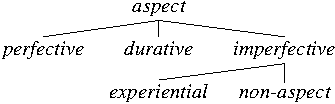
\includegraphics[scale=.8]{pdf/aspect.pdf}
\xe}
\vspace{-20pt}


\noindent The grammatical aspect in Chinese is largely expressed by
verbal markers. There are three aspectual markers in Mandarin Chinese:
\CJK{UTF8}{gkai}{了} \textit{l\`{e}}, \CJK{UTF8}{gkai}{着}
\textit{zh\`{e}} and \CJK{UTF8}{gkai}{过} \textit{gu\`{o}}. They are
respectively responsible for perfective, durative, and experiential.
Since each verb lexically selects these markers, not all these three
items can be necessarily attached to all verbs. For example, 去 q\`{u}
`go' does not canonically co-occur with zh\`{e}. These markers are
collectively know as \textsc{le-zhe-guo} or LZG, and they are
hierarchically constrained as descibed in \myref{tdl:lzg}. 

{\small 
\ex<tdl:lzg>
\texttt{
+vjp :+ [ LZG lzg ].\newline
\mbox{ }lzg := avm. \newline
\mbox{ }le := lzg.\newline
\mbox{ }zhe := lzg.\newline
\mbox{ }guo := lzg.\newline
\mbox{ }no-lzg := lzg.\newline
\mbox{ }le+zhe := le \& zhe.\newline
\mbox{ }le+guo := le \& guo.\newline
\mbox{ }zhe+guo := zhe \& guo.\newline
\mbox{ }le+zhe+guo := le \& zhe \& guo.}
\xe}
\vspace{-20pt}

The \textsc{le-zhe-guo} markers are also restricted in their
co-occurrence with \anota, either with the entire {\anota} phrase, or
with the individual \textsc{A} elements. The first two markers are not
allowed to co-occur with {\anota} at all, while \textit{gu\`{o}} can
only occur with {\anota} if the \textsc{not} element is
\CJK{UTF8}{gkai}{没} \textit{m\'{e}i}. Using Type Definition Language
(TDL), LZG is 


%\footnote{As the present paper deals only with the \textit{bu} form of
%\anota, we will not delve further.}



\subsection{Character}
\label{ssec:char}

To recall from \S\ref{sec:properties}, the $A$ elements in {\anota} are
full or partial reduplicates of each other. One such form is that only
the first character of {\aone}  is reduplicated. With this in mind, we
introduced four new feature types to the lexicon entries, as presented
in (\getref{avm:vjp}):

{\small 
\ex\deftagex{avm:vjp}
\vspace{-10pt}
\newline
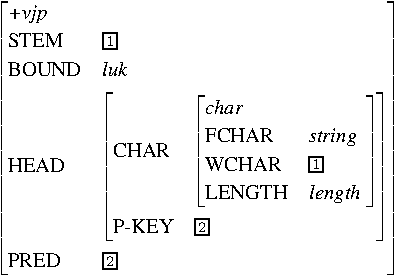
\includegraphics[scale=.8]{pdf/vjp.pdf}
\xe}
\vspace{-20pt}

The feature types \textsc{wchar} and \textsc{fchar} specify the whole
character and the first character of a lexical entry, respectively. The
feature \textsc{wchar} is identical to the \textsc{stem} of the lexical
entry. Next, the \textsc{length} specifies that an entry has
\textit{one} or \textit{more-than-one} character. Finally, the \tdl{luk}
feature \textsc{bound} specifies if an entry is a bound or non-bound
form.\footnote{The \tdl{luk} constraint consists of three components,
such as \ensuremath{+}, \ensuremath{-}, and \tdl{na}
(not-applicable).} This is to ensure that one-character {\aone}  forms
of a multi-character word are used outside of \anota, as they are not
independent morphemes. 


To provide a clearer idea, the entries in (\getref{avm:xihuan})
illustrate the bound and non-bound forms of \CJK{UTF8}{gkai}{喜欢},
respectively. As they are identical to each other apart from length,
they take the same \textsc{pred} value.

{\small 
\pex<avm:xihuan>
\a<xi>
\vspace{-10pt}
\newline
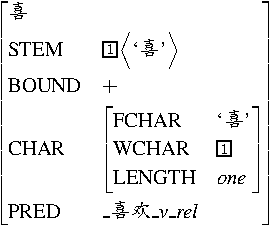
\includegraphics[scale=.8]{pdf/xi.pdf}
\a<xihuan>
\vspace{-10pt}
\newline
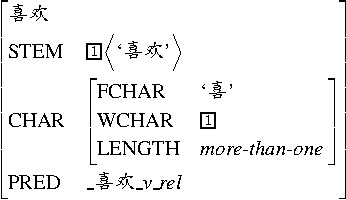
\includegraphics[scale=.8]{pdf/xihuan.pdf}
\xe}
\vspace{-20pt}



\subsection{AVM}
\label{ssec:avm}




{\small 
\ex\deftagex{avm:super}
\vspace{-10pt}
\newline
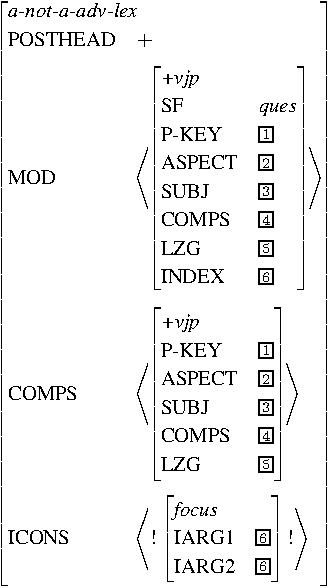
\includegraphics[scale=.8]{pdf/super.pdf}
\xe}
\vspace{-20pt}



{\small 
\pex<avm:neg>
\a<bu>
\vspace{-10pt}
\newline
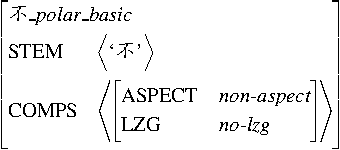
\includegraphics[scale=.8]{pdf/bu.pdf}
\a<mei>
\vspace{-10pt}
\newline
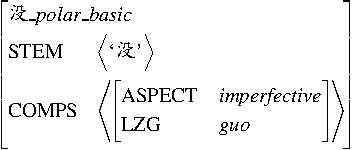
\includegraphics[scale=.8]{pdf/mei.pdf}
\xe}
\vspace{-20pt}


\section{Different Forms of {\anota} Questions}
\label{sec:forms}


\begin{figure*}[!t]
\centering
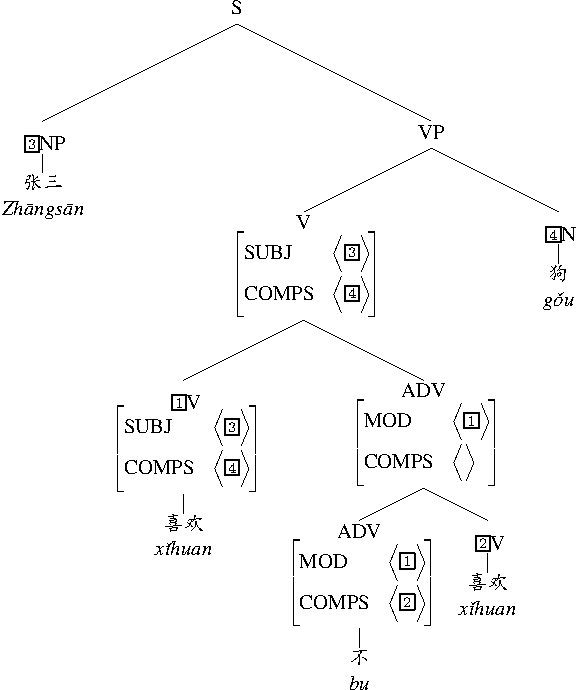
\includegraphics[scale=.8]{pdf/tree1.pdf}
\mbox{ }~\mbox{ }~\mbox{ } 
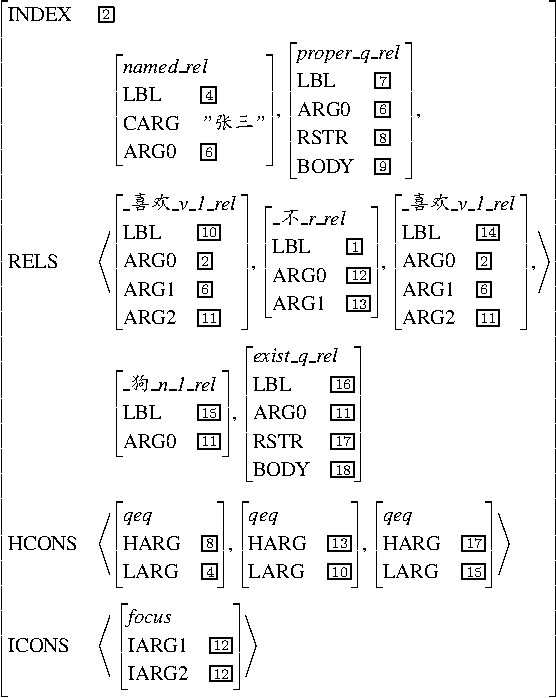
\includegraphics[scale=.8]{pdf/mrs.pdf}
\caption{A sample derivation}
\label{fig:tree1}
\end{figure*}




\subsection{\textsc{A-not-A}}
\label{ssec:basic}




{\small 
\ex\deftagex{avm:basic}
\vspace{-10pt}
\newline
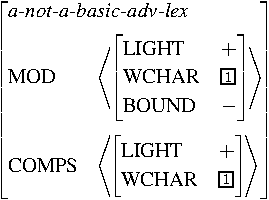
\includegraphics[scale=.8]{pdf/basic.pdf}
\xe}
\vspace{-20pt}


%% {\small 
%% \ex\deftagex{fig:tree}
%% \vspace{-10pt}
%% \newline
%% 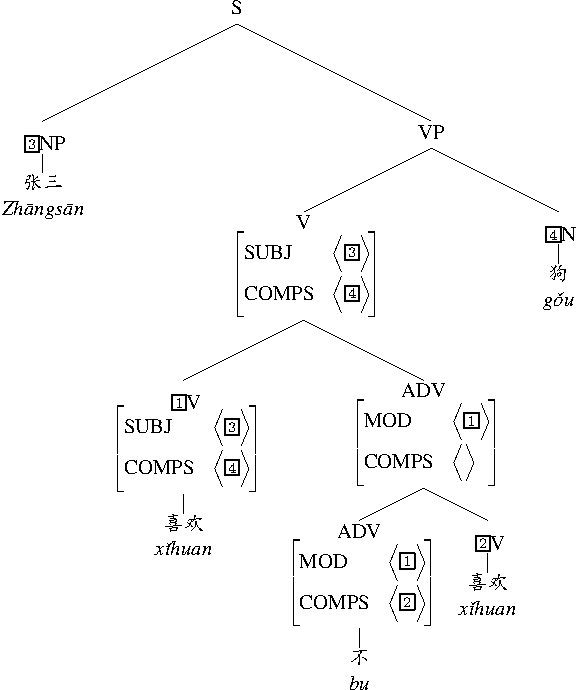
\includegraphics[scale=.8]{pdf/tree1.pdf}
%% \xe}
%% \vspace{-20pt}


%% {\small 
%% \ex\deftagex{avm:mrs}
%% \vspace{-10pt}
%% \newline
%% 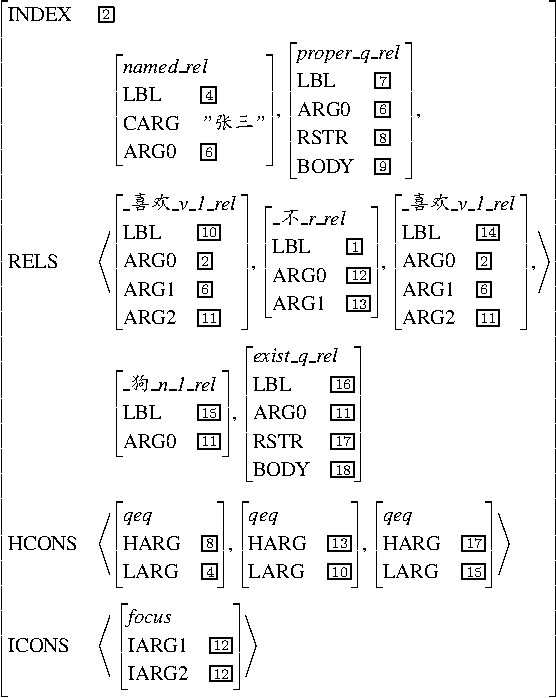
\includegraphics[scale=.8]{pdf/mrs.pdf}
%% \xe}
%% \vspace{-20pt}








{\small 
\CJK{UTF8}{gkai}{
\pex<exe:out>
\a<a> \ljudge*
\begingl[glspace=.5em]
\gla 张三 讨厌 不 喜欢 狗 ?//
\glb Zh\={a}ngs\={a}n taoy\`{a}n b\`{u} xihu\={a}n gou ?//
\glc Zhangsan hate \textsc{not} like dog \textsc{pu}//
\glft `(lit.) Does Zhangsan hate or not like dogs?'//
\endgl
\a<b> \ljudge*
\begingl[glspace=.5em]
\gla 张三 喜 不 喜 狗 ?//
\glb Zh\={a}ngs\={a}n xi b\`{u} xi gou ?//
\glc Zhangsan like \textsc{not} like dog  \textsc{pu}//
\glft `Does Zhangsan like or not like dogs?' // 
\endgl
\xe}}
\vspace{-20pt}



\subsection{\textsc{A\ensuremath{^\prime}-not-A}}
\label{ssec:contracted}




{\small 
\ex\deftagex{avm:contracted}
\vspace{-10pt}
\newline
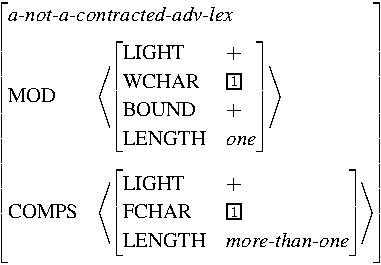
\includegraphics[scale=.8]{pdf/contracted.pdf}
\xe}
\vspace{-20pt}



\subsection{\textsc{AB-not-AB}}
\label{ssec:phrasal}




{\small 
\ex\deftagex{avm:ab}
\vspace{-10pt}
\newline
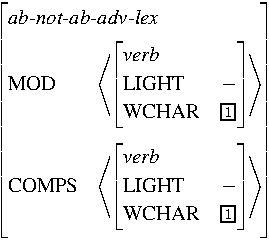
\includegraphics[scale=.8]{pdf/ab.pdf}
\xe}
\vspace{-20pt}


\section{Implementation}
\label{sec:implemetation}


\section{Evaluation}
\label{sec:evaluation}

gTest 
pyDelphin


HELD-OUT
TEST



%\section{Conclusion}
%\label{sec:conclusion}






\bibliographystyle{acl}
\bibliography{sanghounsong}



\end{document}
